\section{Introduction}

    \subparagraph{}Le but de ce {\color{info}4\ieme{} travail} est de réaliser un circuit avec au minimum 4 résistances,
    une source de tension et de courant, une capacité et un interrupteur qui se ferme ou s'ouvre en $t\; =\; 0$ et enfin
    de simuler le circuit avec le logiciel \textit{LTspice} afin de démontrer l'exactitude des calculs.\\[1.5cm]
    
    \begin{titletbox}{À l'attention du correcteur / correctrice}{warning}
        N'hésitez pas à zoomer sur les schémas du circuit et autres images afin d'y voir plus clair.
    \end{titletbox}

\section{Schéma initial du circuit}

    \begin{figure}[H]
        \centering
        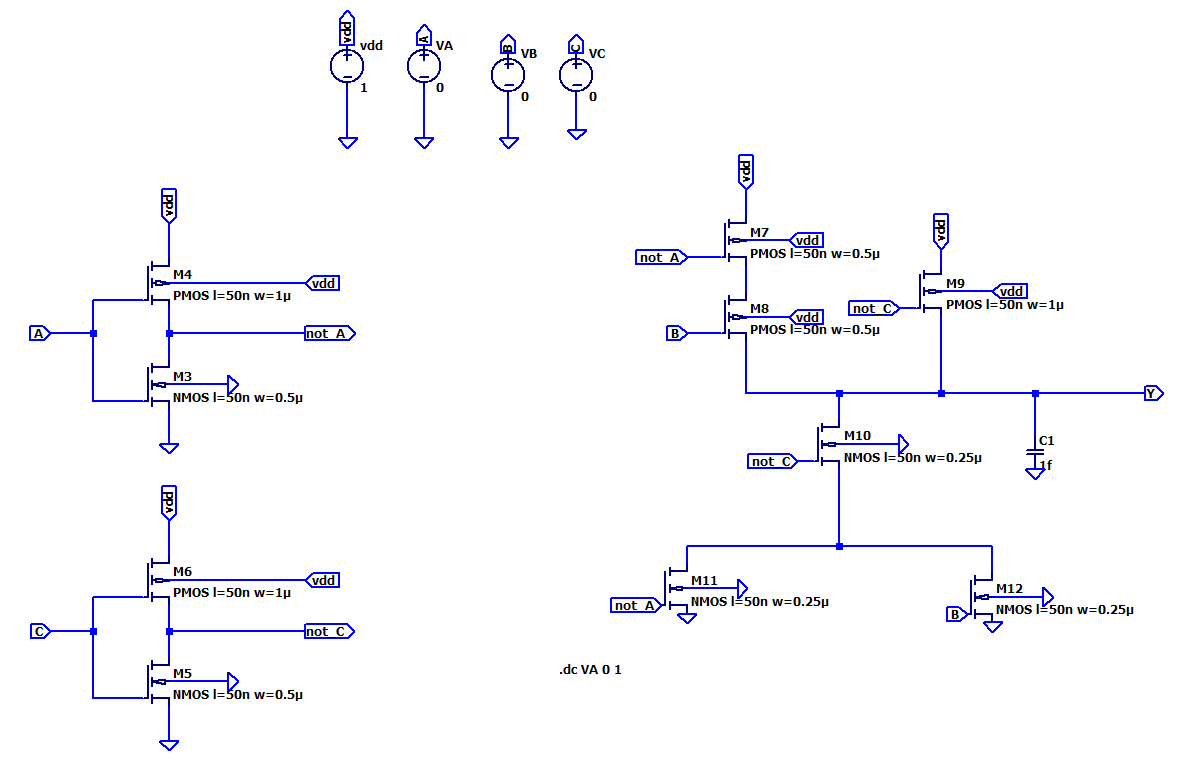
\includegraphics[scale=0.5]{../pictures/circuit.png} % Pas utiliser width=\textwidth pcq il prend la taille de \section{} comme ref
        \caption{Schéma du circuit}
    \end{figure}

    \section{Calcul de la condition initiale : $V_C(t\leq0)$}

    \subparagraph{}Comme l'interrupteur est ouvert en $t\leq0$ et que la capacité se comporte comme un circuit ouvert, j'obtiens le morceau suivant :
    
        \begin{figure}[H]
            \centering
            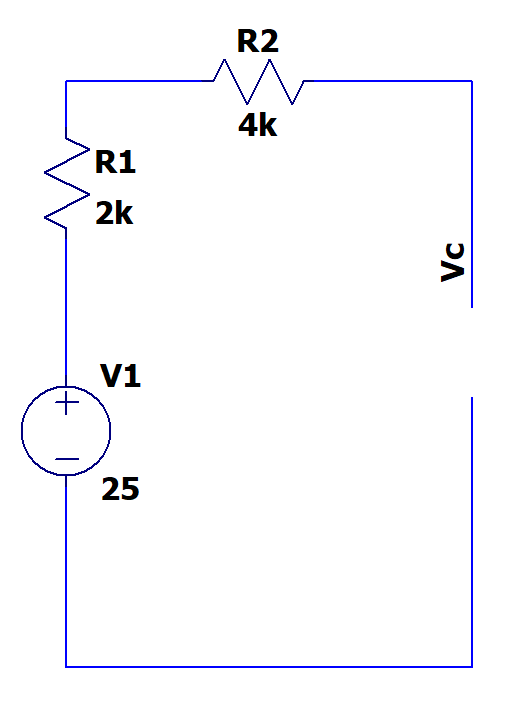
\includegraphics[scale=0.5]{../pictures/open.PNG}
            \caption{Circuit en condition initiale}
        \end{figure}
        
        
    \subparagraph{} Dès lors, n'ayant pas de courant, on peut directement déterminer que la tension aux bornes de la capacité vaut 25 volts
    
    \begin{empheq}[box=\fbox]{equation*}
    \color{red}
        V_C (t\leq0)\;=\;25\;V
    \end{empheq}

\section{Calcul de la condition finale : $V_C(t=\infty)$}
    
    \subparagraph{}En condition finale, l'interrupteur est fermé et nous avons donc le circuit suivant :
    
        \begin{figure}[H]
            \centering
            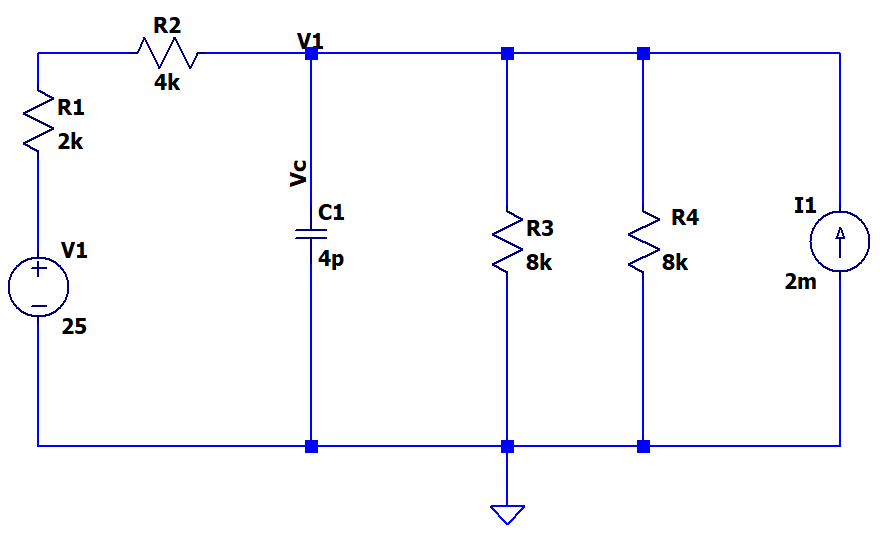
\includegraphics[width=0.7\textwidth]{../pictures/close.PNG}
            \caption{Circuit en condition finale}
            \label{fig:final}
        \end{figure}
        
        
    \subparagraph{}Grâce à la loi des noeuds, nous pouvons poser l'équation suivante pour trouver $V_1$ :
    
        \begin{equation*}
            \color{info}
            \frac{25\;-\;V_1}{6k}\;+\;2m\;=\;\frac{V_1}{8k}\;+\;\frac{V_1}{8k} 
        \end{equation*}
        
        \begin{equation*}
            \color{info}
            \frac{25\;-\;V_1}{6000}\;+\;\frac{1}{500}\;=\;2 \cdot \frac{V_1}{8000}
        \end{equation*}
        
        \begin{equation*}
            \color{info}
            74\;-\;2 \cdot V_1\;=\;3 \cdot V_1
        \end{equation*}
        
        \begin{equation*}
            \color{info}
            V_1\;=\;\frac{74}{5}\;(14,8)\;V
        \end{equation*}
        
    \subparagraph{}Or on sait que $V_1$ = $V_C$ donc :
        \begin{empheq}[box=\fbox]{equation*}
            \color{red}
                V_C (t=\infty)\;=\;14,8\;V
        \end{empheq}
        


\section{Calcul de la constante de temps $\tau$}

    \subparagraph{}La constante $\tau$ peut se calculer via la formule suivant :
    
        \begin{equation*}
            \color{info}
            \tau\;=\;R_{Eq} \cdot C
        \end{equation*}
        
        
    \subparagraph{}Pour trouver la résistance équivalente, on reprend le circuit de la \textbf{figure \ref{fig:final}} où on annule les sources (comme lorsque qu'on cherche la $R_{eq}$ pour un équivalent de Thévenin ou Norton). De plus on sait que la capacité se comporte comme un circuit ouvert ce que nous donne le schéma suivant :
    
        \begin{figure}[H]
            \centering
            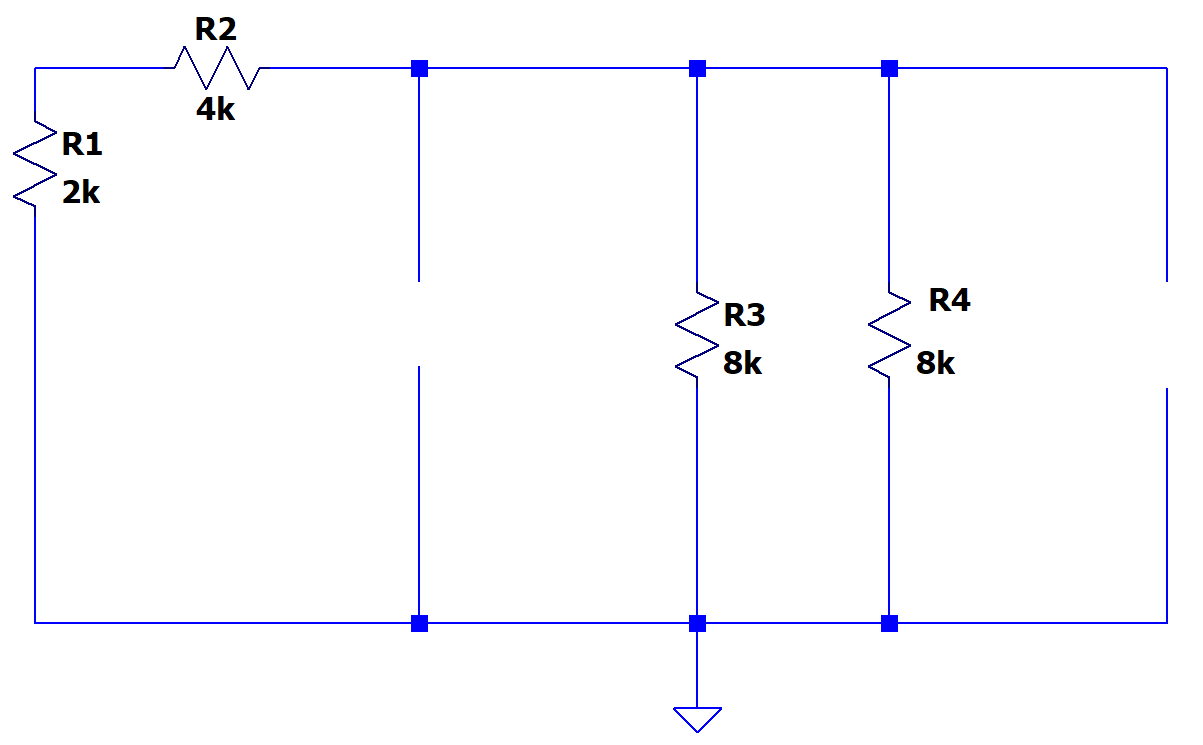
\includegraphics[width=0.7\textwidth]{../pictures/cancel.PNG}
            \caption{Sources annulées}
            \label{fig:my_label}
        \end{figure}
        
        
    \subparagraph{}On a donc (($R_1$ + $R_2$) // $R_3$) // $R_4$ (dans les calculs je note $Ans$ le resultat obtenu au calcul précédent):
    
        \begin{equation*}
            \color{info}
            R_1\;+\;R_2\;= 6\;k\Omega
        \end{equation*}
        
        \begin{equation*}
            \color{info}
            Ans\;//\;R_3= \frac{6 \cdot 8}{6 + 8}
        \end{equation*}
        
        \begin{equation*}
            \color{info}
            Ans\;//\;R_3\;=\;\frac{24}{7}\;k\Omega
        \end{equation*}
        
        \begin{equation*}
            \color{info}
            Ans\;//\;R_4\;=\frac{\frac{24}{7} \cdot 8}{\frac{24}{7} + 8}
        \end{equation*}
        
        \begin{equation*}
            \color{info}
            Ans\;//\;R_4\;=\frac{\frac{24}{7} \cdot 8}{\frac{24}{7} + 8}
        \end{equation*}
        
        \begin{empheq}[box=\fbox]{equation*}
            \color{red}
            R_{eq}\;=\;2,4\;k\Omega
        \end{empheq}
        
        
        \subparagraph{}On peut donc maintenant calculer $\tau$ :
        
            \begin{equation*}
                \color{info}
                \tau\;=\;R_{eq} \cdot C
            \end{equation*}
            
            \begin{equation*}
                \color{info}
                \tau\;=\;2,4\;k\Omega \cdot 4\rho F
            \end{equation*}
            
            \begin{empheq}[box=\fbox]{equation*}
                \color{red}
                \tau\;=\;9,6nS
            \end{empheq}

\section{Tension aux bornes de la capacité $V_C(t)$ pour $t>0$}

    \subparagraph{}On peut calculer la tension suivant la formule suivante :
        
    {\color{info}\begin{align*}
        V_C(t)\;&=\; V_\infty + (V_0 -V_\infty) \cdot \euler^{\frac{-t}{\tau}}\\
        V_C(t)\;&=\; 14,8 + (25 - 14,8) \cdot \euler^{\frac{-t}{9,6nS}}\\
    \end{align*}}

    \begin{empheq}[box=\fbox]{equation*}
        \color{red}
        V_C(t)\;=\; 14,8\;V + 10,2\;V\cdot \euler^{\frac{-t}{9,6nS}}
    \end{empheq}

\section{Courant de la capacité $I_C(t)$ pour $t>0$}

    \subparagraph{}On peut calculer le courant de la capacité suivant la formule suivante :
        {\color{info}\begin{align*}
            I_C(t)\;&=\;C \cdot \frac{dV_C}{dt}\\
        \end{align*}}
        
    \subparagraph{}En résolvant la dérivée, on obtient :
    
         {\color{info}\begin{align*}
            I_C(t)\;&=\;C \cdot 1,133G \cdot \euler^{\frac{-t}{9,6nS}}\\
            I_C(t)\;&=\;4 \cdot 1,133G \cdot \euler^{\frac{-t}{9,6nS}}\\
        \end{align*}}
        
        \begin{empheq}[box=\fbox]{equation*}
            \color{red}
            I_C(t)\;=\;4,533 \cdot \euler^{\frac{-t}{9,6nS}}\;A
        \end{empheq}
        
\section{Simulation du circuit}
        \begin{figure}[H]
            \centering
            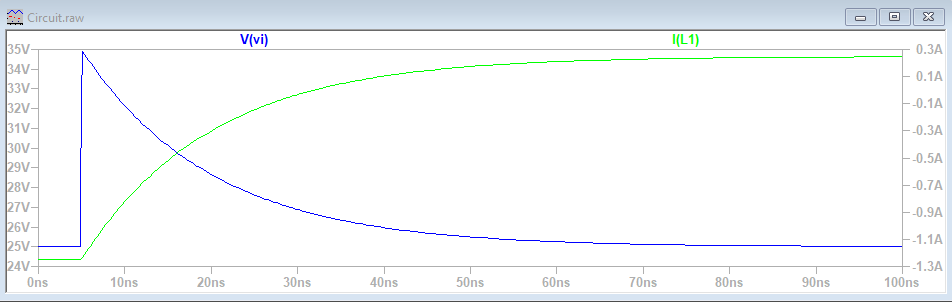
\includegraphics[width=1.05\textwidth]{../pictures/simu.png}
            \caption{Simulation du circuit, avec la tension en bleu et le courant en vert}
        \end{figure}
\section{Conclusion}

    \subparagraph{}Pour conclure ce travail, on peut également voir grâce à la simulation que j'ai 25 volts à la situation initiale et 14,8 volts pour la situation finale, ce qui confirme mes calculs. Le délai de 2 nanosecondes dans mon graphique s'explique par le fait que j'ai explicitement mis un délai dans ma commande PULSE sur $LTspice$.

\end{document}